
\chapter{The Demands of Software}\label{ch:softwaredemands}

\squo{“So many things are possible as long as you don't know they're impossible.”
}{\emph{The Phantom Tollbooth},\\Norton Juster}
\begin{chabstract}
    This chapter will focus on software, the needs of software we must address, and the perspective of systems
    programming, putting the hardware trends we spoke of last chapter into context. We will discuss the problem of
    ephemeral context and discuss how persistence and RPC have shared characteristics and concerns.
\end{chabstract}

At their core, applications perform computation on in-memory data. Yet much application complexity is tied up in the
infrastructure surrounding that computation, for example, in managing persistent state and in performing serialization.
Additional work done by the program (or by the operating system on behalf of the program) that is merely in service of
setting up the computation and not the computation itself is considered \emph{overhead}. Our goal is to
reduce that overhead in two ways: improving performance and reducing complexity. To do this, we need to understand where
overhead comes from, which elements are fundamental, and which are not.

\squo{One goal in designing and implementing an operating system is to
    provide high performance; another way to say this is our goal is to minimize the overheads of the OS. Virtualization and making the system easy
    to use are well worth it, but not at any cost.}{Operating Systems:\\Three Easy Pieces~\cite{ostep}}
\section{The Old Ways and ``Systems Programming''}

Current operating system interfaces are a poor fit for the trends and hardware requirements we discussed last chapter.
File \texttt{read} and \texttt{write} interfaces, originally designed for sequential media and later expanded for
block-based media, require significant kernel involvement and often serialization, violating both the requirement to reduce
kernel involvement, and the need to reduce the length of code paths around accessing data. Figure~\ref{fig:cycle} shows a fairly
common data path for an application that operates on (and perhaps mutates) some persistent data. First the data is
loaded explicitly into memory, either in a streaming fashion or as a whole file, followed by the application manually
deserializing it into an in-memory form. Once this is done, the program may commence its actual purpose---to perform
computation---after which the results are serialized and placed back onto disk with an explicit store operation.

\begin{SCfigure}
    \centering
    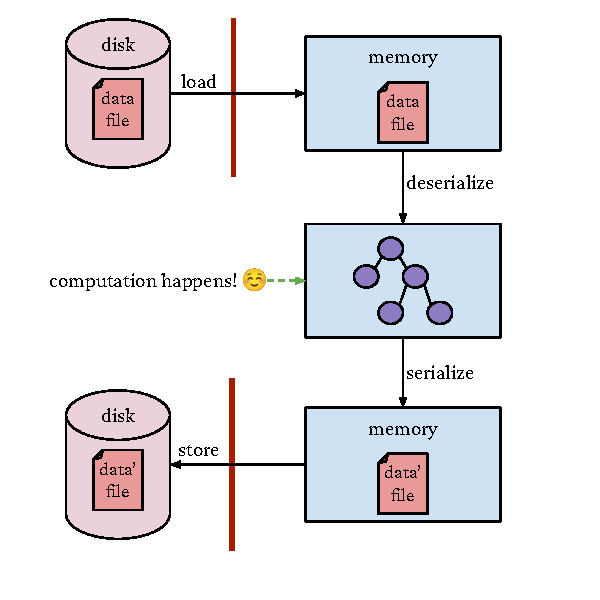
\includegraphics[width=\linewidth]{fig/cycle.pdf}
    \caption[The cycle of systems programming]{The ``standard cycle'' of systems programming. We start with some persisted data, explicitly load it from disk into memory, deserialize it, compute on it, reserialize it, and explicitly store it back to disk. Note that the vast majority of this diagram depicts stuff other than the actual computation. The thick red lines depict persistence boundaries, across which data exists in different contexts and assumed lifetimes.}
    \label{fig:cycle}
\end{SCfigure}

Let's consider the case from Chapter~\ref{ch:farout} of faster, closer persistence.
In the past, the overhead in manually loading and unloading
data and in transforming it to and from an on-disk form was acceptable, since the cost to access the disk was high,
and those explicit load and store disk operations were going to be issued anyway. But when these operations overshadow
%% TODO cite more examples
device access time, the overhead quickly becomes unacceptable. As devices become faster and as applications process more
and more data, we find that more and more of our processing time is spent here. Applications can spend as much as 70\% of the processing
time~\cite{trims} deserializing and loading data into main memory at request time. Reducing this overhead would save
both in program time but also in \emph{programmer} time. Simplifying applications by removing serialization
helps programmers by removing the need to maintain multiple data formats and the transformation code to move data
between those formats.

\subsection{The Context Problem}

If we look closely, the cycle in Figure~\ref{fig:cycle} can represent more than just processing files. It works
equally well for receiving data from a network and sending back a response (microservices and servers in general), or for
applications in a traditional \texttt{pipe}line, \etc\sidenote[][-1in]{\footnotesize Those who sit high atop their \unix throne claim that text is a universal communication language. Yet anyone
    who has actually had the misfortune of parsing the output of even a moderatly complex \unix tool can realize that
    systems programming here involves just as much serialization and processing work as anywhere else---or else involves
    doing computation directly on C strings, a fate I would not wish upon my worst enemy.
}. But why do we often spend so much time and effort with serialization and explicit I/O? Because the POSIX abstractions
fundamentally bifurcate our programming model into two separate \emph{contexts}:

\begin{enumerate}
    \item \textbf{Local Context} contains data that is limited to a single domain, for example in-memory data accessed
          via virtual addresses by a single process, or the domain of file descriptors. Data in a local context is typically
          operated on ``directly'' since it's usually in memory. Most importantly, though, the data isn't \emph{shared} with
          other domains, and it is ephemeral---its lifetime is tied to the context it is in.
    \item \textbf{Global Context} contains data that is shared across all the domains. Typically this covers data stored
          on disk or other stable storage. Data in a global context is usually stored in some serialized format and can
          be accessed by multiple domains simultaneously. The lifetime of data herein is, in the limit,
          infinite\sidenote{Even in the global context, we traditionally separate local storage and network storage.
              That separation can be eroded depending on the programming model, however, as we will discuss later.}.
\end{enumerate}

These separate contexts give rise to the need to transform data between them and to be explicit about marshalling data
across the boundary. The primary reason for the need for transformation has to do with \emph{data references} and
\emph{naming data}. For example, when applications operate on in-memory data, references take the form of virtual
addresses---pointers refer to specific locations within the virtual address space. The virtual address space is
ephemeral---it's tied to a specific process. But \emph{persistent} data is \emph{not} ephemeral! By definition it is
accessed by multiple processes, either over time (different invocations of the same process), or across space (shared
between multiple processes), or both. In either of these cases, virtual addresses cannot be used, since those addresses
may not agree across different contexts. So when sharing memory, any references to local context data must be
transformed into something that can be interpreted within the global context.

More generally, we often lock data access behind context that is tied to a shorter-lifetime actor, leading to
unnecessary indirections and extraneous work that the program must perform.
This is illustrated in how data relationships are typically handled, either:
\begin{enumerate}
    \item \textbf{Explicit, context-sensitive.} As we saw with virtual address pointers,
          references between data are encoded explicitly but rely on context provided by
          the ephemeral process abstraction. These references cannot be reliably shared between
          applications and across nodes which do not have the context necessary to interpret them.
    \item \textbf{Implicit.} Many data relationships are implicit in applications.
          Although there is a relationship between the \unix files \texttt{/etc/shadow} and \texttt{/etc/passwd},
          it is not explicit. This limits interoperability between programs, prevents
          relationship discovery, and results in a brittle environment if these files are
          moved or replaced.
    \item \textbf{Explicit, via mediators.} Relationships can be encoded explicitly without
          ephemera if we use a global name resolution service. For example, an HTML
          file can refer to a style sheet by name. However, this presupposes the existence (and
          availability) of a global mediator and restricts programs from agreeing on the identity
          of data behind a reference without complex inter-networking and expensive global coordination.
\end{enumerate}

In our view, the complexity of these mechanisms is a symptom of a more fundamental problem: access to long-lived data
is unnecessarily mediated via ephemeral actors.
We advocate a violent break from this actor-centric model of data access, in favor of a model that elevates \emph{data}
as the systems' first-class citizen.  Doing so will require \emph{explicit
    context-free} references via globally unique identifiers (GUIDs) that name data objects. These
references are independent of context (\eg process) that operates on them, and require that all context necessary to interpret references
be stored within the data itself. Of course, we still need some understanding of
context-sensitive relationships, for example late-binding of names. We do this via a
``two-level'' naming system in which GUIDs are \emph{authoritative} names to which we can bind
additional names for purposes like local references, changing data identification, and discovery\sidenote{We will
    discuss these in more detail in Chapter~\ref{ch:invariant}.}.
%\sidenote{See Section~\ref{sec:latebinding}.}.

Viewing the past through the lens of the present, it was \emph{always} a mistake to entangle the context required to access
and manipulate data with ephemeral actors.  However, in the days of slow networks, spinning disks and small memories,
it was possible to hide these complexities and inefficiencies.  For one thing, disk-based I/O led to a model of sharing in
which long-lived data and computable data were stored in different \emph{kinds} of memory, in different formats (due to serialization),
with different reference formats (e.g., file names vs. virtual memory pointers).
The filesystem was a natural location to place the various hacks that were required to paper over the reality
that interacting with long-lived data required figuring out how to name the short-lived processes that were the primary
citizens of the operating system.

Needless to say, a disaggregated system model---one in which a particular data reference may
ultimately point to data on a different node from the one observing the reference---exacerbates all of these problems!
Two different nodes that observe the same data reference should agree on what data is
being referred to, and by the same token, an individual node observing two different data references
should be able to determine if they point to the same data. This asks the question of \emph{how}
to encode these explicit context-free data references while remaining efficient and avoiding global
coordination\sidenote{We will discuss and answer these questions in detail in Chapters~\ref{ch:global} and \ref{ch:invariant}.}.


\section{Retrofitting POSIX?}

While I am arguing strongly that a clean-break reimagining is needed, it is worth considering what an incremental
approach might look like. For example, the problem of direct access might be solved to some extent by \texttt{mmap}, the
problem of global references could be solved by traditional pointer swizzling built atop \texttt{mmap}, \etc. We could
even combine this with RDMA to gain a \ac{dsm} model.

Let's first consider the use of \texttt{mmap} to provide an interface for \NVM before looking more broadly at
persistence in general.
The \texttt{mmap} system call attempts to hide storage behind a memory interface through hidden
data copies. But, with \NVM, these copies are wasteful, and \texttt{mmap} still has significant kernel
involvement and the need for explicit \texttt{msync} calls. ``Direct Access'' (DAX)
tries to retrofit \texttt{mmap} for \NVM DIMMs by removing the redundant copy, but this \emph{still}
fails to address the problem of global context and in-memory data structures for persistent storage.
Operating on persistent data through \texttt{mmap} requires the programmer to
use either fixed virtual addresses, which presents an infeasible coordination problem
as we scale across machines and is fundamentally unportable, or virtual addresses directly, which are ephemeral and require the
context of the process that created them\sidenote{These issues don't even touch the high kernel
    involvement, in-kernel coordination, and failure-atomicity hazards present when using \texttt{mmap}~\cite{crotty22-mmap}.}.

Attempting to shoehorn \NVM programming atop POSIX interfaces (including \texttt{mmap}) results in
complexity that arises from combining multiple partial solutions. Given some feature desired by an
application, the \NVM framework can provide an integrated solution that meshes
well with the existing support for persistent data structure manipulation and access, or it can
fall-back to POSIX resulting in the programmer needing to understand two different ``feature
namespaces'' and their interactions. An example is naming, where a programmer may need
to turn to the filesystem to manage names in a completely orthogonal way to how the \NVM framework handles
data references. For example, PMDK, an \NVM programming library, relies on a filesystem for naming and initial access to
persistent memory objects, resulting in different kinds of references, feature sets from filesystems
being applied (like security) while others are not (data access), and the complexity of
understanding how the PMDK abstractions interact with the POSIX ones. Instead, our model prefers to
build legacy support atop new abstractions (as we will see in Section~\ref{sec:legacy}), and avoid falling back to legacy
models for persistent data access.

Even without \NVM, we have similar problems. Our goal of programming with memory semantics on in-memory data structures
leads to many of the same arguments as above.
Additionally, systems that layer new models atop existing interfaces often fail to facilitate effective persistent data sharing and
protection.  PMDK, for example, makes design choices that limit
scalability, since its
data objects are not self-contained and do not have a large enough ID space, resulting
in the need to coordinate object IDs across machines, a problem we will explore in detail in Chapter~\ref{ch:global}. For the same reason,
although single-address space OSes~\cite{chase:tocs94} somewhat address our requirements, they do
not consider both requirements at once, nor do they provide an effective and scalable solution to
long-term data references due to that same coordination complexity (as we will discuss in Section~\ref{sec:historical}).




\section{Remote Procedure Calls}

One major aspect of systems programming, particularly in distributed systems, is RPC\sidenote{Note that, if you look at
    Figure~\ref{fig:cycle} and squint your eyes, it resembles not just persistence but also communication and data
    transfer across nodes.}. We typically use RPC as a mechanism for decomposition in distributed systems, allowing us
to break design problems down into smaller, re-usable parts that hide implementation details and are more easily debugged.
Decoupling components with RPCs allows them to scale
independently---in principle, developers need only agree
on a common interface and message format to leverage the
benefits of software decoupling. Yet, in reality,
RPCs enforce strict interface constraints and often
trade adaptability (narrow interfaces are harder to evolve) for
simplicity (narrow interfaces limit cross-component interactions),
ultimately hampering the goal of scalability.


The chief problem with RPCs is that they are fundamentally location-
and compute-centric: RPCs force a
programmer to decouple an application by explicitly separating the
computational endpoint or \emph{location} where a function is invoked
from the location where the function executes.  As a consequence, they are
well-suited to a relatively narrow set of use cases in which
function arguments, which flow from invoker to executor, and
returns, which flow back, must be serialized and sent in their
entirety, and hence are small, and in which reference data must be
located on the executor.


Many scenarios would benefit from decoupling but are simply not feasible using existing RPC
mechanisms. For example, the invoking endpoint may have abundant data but limited
compute, the invoker may wish to traverse a remote data structure, or the invoker may wish to
refer to data that they lack privileges to read. Rapidly growing model sizes, privacy concerns, and the proliferation of last-mile
model customizations all exacerbate the issue.
To mitigate the problem of location-centric RPCs, data center
operators often deploy discovery services, load balancers, or other
forms of middleware~\cite{eisenbud16,katran,tibco,kreps11,mq}. These
extra indirection layers make the execution endpoint abstract, but at
the cost of increased latency and added system complexity. Moreover,
we argue that such systems do not address the fundamental problem,
which is that \emph{we need a more general mechanism for module
    composition in distributed systems}.

\subsection*{Motivating Example}

To illustrate the poor fit of RPC as a decoupling mechanism for some classes of applications,
consider the problem of distributed inference for edge devices. Here,
sensors in mobile devices with modest processing and storage resources (\eg mobile phones)
are the source of observations used both for training and inference.
Recent work has focused on decoupling and distributing machine learning training across edge
and cloud resources to minimize client-perceived latency, provide privacy guarantees, and
maximize server-side throughput~\cite{federatedml,singh2019detailed}.

In this example, we focus on the inference problem that arises in response to device input.
Ideally, small models trained in the
cloud (via a methodology such as federated learning) are periodically shipped in their entirety to
edge devices, which perform local inference.  Several trends are upsetting this model. The first
is the aggressive growth---roughly 10$\times$/year---of models, in particular language models.
In 2018, the largest machine translation models at Google were 8.3 billion
parameters~\cite{megatron}; a mere two years later, the largest models exceeded 800 billion parameters!
Inference on sparse giant models which far exceed device resources must be performed server
side, where model serving presents a substantial throughput bottleneck. This is further
compounded by last-mile model customization for end users, in which inference tasks
for different devices \emph{must} be performed on slightly different models.  As much as 70\%
of the processing time~\cite{trims} for these model-serving applications is spent deserializing
and loading the sparse personalized models into main memory at request time. Finally, users prefer
local models remain local due to confidentiality concerns.

Consider a concrete example (Figure~\ref{fig:rpccopy}) that is bedeviled by all of these complexities at once. A mobile device,
Alice, in possession of a locally-trained model and an activation, wishes to perform a
classification task that requires a partition of a sparse global model, located on cloud resource
Bob. Further, imagine that Alice cannot perform the inference locally, either because the global
model fragment is too large or because she has inadequate local compute. Finally, imagine that Bob
is overloaded, while a separate cloud resource, Carol, is mostly idle.


\begin{SCfigure}
    \centering
    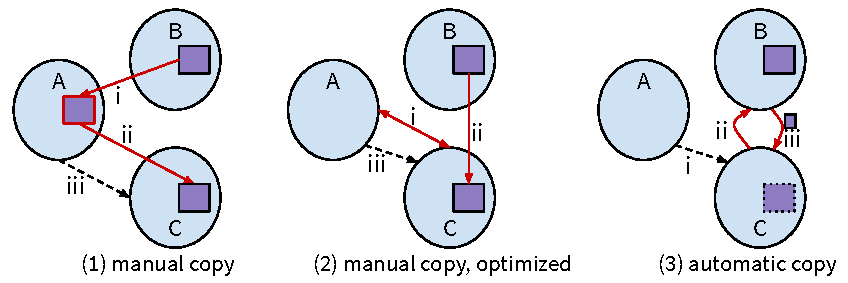
\includegraphics[width=\linewidth]{fig/copy}
    \caption[Rendezvous of data and compute]{Rendezvous of data and compute. Solid red arrows are additional
        infrastructure-level tasks that are not fundamental to the requested computation.}
    \label{fig:rpccopy}
\end{SCfigure}

An ideal solution will minimize the latency Alice perceives and maximize the throughput offered
by both Bob and Carol, all while satisfying capacity constraints of each. It is easy to see
that while this application requires decoupling, RPC is the wrong abstraction in terms of performance,
expressivity, and flexibility.  Data movement---whether from storage to DRAM on Bob or from Bob
to Carol---requires costly serialization. If moving the data to Carol and performing
inference there is the optimal solution, the application logic on Alice must orchestrate this
infrastructure-level concern, either by pushing the data through Alice (Figure~\ref{fig:rpccopy} (1), a na\"ive solution)
or having the RPC executed
on Carol address Bob directly and pull (Figure~\ref{fig:rpccopy} (2)).
Both (1) and (2) require additional logic on Alice
to work---the programmer had to perform the infrastructure level task of data
movement.  Fundamentally, these issues arise because the system's core abstraction is
location-based---the programmer is forced to manually orchestrate machines or resort to
costly copying\sidenote{Additionally, there are issues of security and coordinating topology changes.}.
Further,
heterogeneity among end devices makes the ``hard-coded'' data movement strategy
brittle:
a subsequent classification request from client device Dave will be forced to run inference
on the server side even if it is equipped with the resources to do the work locally.

Figure~\ref{fig:rpccopy} (3) is more ideal. The first step is for
the computation to move to Carol instead of first moving data in preparation.  This may seem like a
minor point, but it is not---by specifying \emph{up-front} the computation we want to perform, we
open the door for lower-level optimization to examine our requests before we go around manually
moving data.  In fact, the programmer may not be directly asking Carol to perform the
computation; instead the placement decision would be made by the system. Once the code starts
executing, we can then move data on demand instead of having to move the entire
object.
Note that this matches the same requirements we discussed above with respect to context---data references must
be \emph{context-free} and global. With the ability to name data in a global context, we not only reduce the need for
serialization, but we also gain the ability to pass by \emph{reference} instead of by value.


\paragraph*{Patterns of RPC.}
%
While RPC is a poor fit here, there are applications for which RPC provides adequate decoupling.
RPC shines in situations where decoupling in the application meshes well with having little data
movement, where an RPC endpoint either fronts large data, large compute relative to the invoker, or
some combination, with \emph{small} arguments and return \emph{values}.
But call-by-small-value is a significant constraint, and there are many
classes of applications that do not fit.
We cannot paper over this problem, either.
Because
RPC is disconnected from a global notion of data identity, we either \emph{cannot} do
call-by-reference (because references must cross machine boundaries) or we must shoehorn this
functionality into the application logic and the RPC's APIs, resulting in brittle, repetitive,
complex code to deal with the coordination, caching, and prefetching that
comes from distributed data and global references when data moves.

The ``good'' use cases of RPC are ones in which code and data
co-location has already been preordained by initial decoupling (after which it is rigid) and
data transfer is minimal---often manifesting as something like a fronted key-value store service. This restricts
code mobility (as it accounts for no change to decoupling later), and requires a myriad of RPC calls
to implement all the ways a programmer might wish to view data (one need only look at the many S3
APIs available as an example).
If we limit ourselves to traditional RPC, any situation (such as the one discussed
above) that does not fit this pattern either results in expensive data movement
and complex application logic, or it must be dismissed altogether and the application redesigned.
By allowing applications to pass data references instead of just values, and by making data
references a first-class abstraction in the OS and the network, applications become much simpler to
express efficiently, even for what would be considered pathological cases for RPC.

\paragraph{A Counter to a Defense of Serialization}

A common response at this point is to point out that serialization serves several other purposes, such as ensuring
portability between environments that use different definitions of (\eg) \texttt{int} in C, or different machine
architectures that differ in endianess. I find these defenses weak. Firstly, for worrying about different ABI of types,
this is already a problem when sharing memory, and is a solved one. Many languages offer support for fixed-width values
and have explicit FFI functionality\sidenote{And continuing in the modern day with C's type system is a complete misstep
    anyway.}. As for endianess, much of the modern world uses little endian, and places that use big endian (networks) don't
really care about the data they are passing, they just worry about protocol headers. In any case, both of these issues
are problems that we can (and regularly do) solve at the language level.

And furthermore, there is nothing fundamentally tying these elements to the idea of global context and references, so
even if they weren't concerns at all, we would still often need to serialize data as it moves across contexts. Our approach
is to solve the fundamental context problem that motivates serialization now, and solve the smaller problems that got
mixed into serialization at a higher level.

\squo{In the early days, building computer systems was easy. Why, you ask?
    Because users didn’t expect much. It is those darned users with their
    expectations of “ease of use”, “high performance”, “reliability”, etc., that
    really have led to all these headaches. Next time you meet one of those
    computer users, thank them for all the problems they have caused.}{Operating Systems:\\Three Easy Pieces~\cite{ostep}}



\begin{chconc}[So, What Does This All Mean (part 2)?]

    Software is growing in complexity, software is becoming more and more distributed with higher and higher demand for
    concurrency as it is asked to process more and more data.
    As we saw both with accessing persistent data and in RPC, serialization takes a huge amount of processor time and a
    large chunk of an application's complexity budget. Relying on kernel crossings to perform I/O is costly, particularly if
    we reduce or remove the need for serialization. Having to resort to call-by-small-value when trying to effect
    computation remotely severely limits the expressability of distributed applications, and can have a negative impact on
    decoupling and modularity---the very thing that RPC is supposed to solve.

    If we are to provide a solution by way of a new programming model and OS abstractions, it must be one that both solves
    the problems that software has and provides abstractions that best take advantage of the new hardware. Mere incremental
    change will not get us there. Fortunately, what we are seeing is a confluence of software demands and hardware trends.
    The hardware is becoming better equipped to support high concurrency, distributed applications that can share memory
    within a larger context. To take best advantage of hardware, we must reduce kernel involvement and move towards a global
    address space of in-memory data---which is exactly the solution that cuts down the overhead of serialization and system calls
    to zero. The remainder of this thesis will discuss how we can use this global address space, with first-class support
    for references, to solve not only the problems of persistence and the systems programming cycle, but also that of
    computation mobility, factoring out complexity, and providing simpler, higher performance applications. But to do
    this, we will need an operating system built for that purpose.

\end{chconc}